\section{Resultados}
    \subsection{Verificación de supuestos}
        La Tabla \ref{supuestos} resume las dos primeras hipótesis. Los tres sectores 
        cumplen el supuesto de normalidad, lo que permite emplear pruebas paramétricas, 
        en cambio, la homogeneidad de varianzas se rechaza de forma contundente.

        \begin{table}[H]
            \centering
            \caption{Normalidad y homogeneidad de varianzas}
            \begin{center}
                \begin{tabular}{|l|l|c|c|}
                    \hline
                    \textbf{Prueba} & \textbf{Grupo} & \textbf{Estadístico} &
                    \textbf{$p$} \\
                    \hline
                    Shapiro-Wilk & Residencial & 0,9912 & 0,7628 \\
                    \hline
                    Shapiro-Wilk & Comercial   & 0,9868 & 0,4246 \\
                    \hline
                    Shapiro-Wilk & Industrial  & 0,9933 & 0,9069 \\
                    \hline
                    Levene (Python)  & Los 3 sectores & 60,43  & $<0{,}001$ \\
                    \hline
                    Bartlett (R)     & Los 3 sectores & 199,39 & $<0{,}001$ \\
                    \hline
                \end{tabular}
                \label{supuestos}
            \end{center}
        \end{table}

        La heterocedasticidad se evidencia en el aumento de la desviación 
        estándar, de 40,6 kWh en Residencial a 195,3 kWh en Industrial, 
        por ello, la comparación de medias se realiza mediante la corrección 
        de Welch.

        \begin{figure}[H]
            \centering
            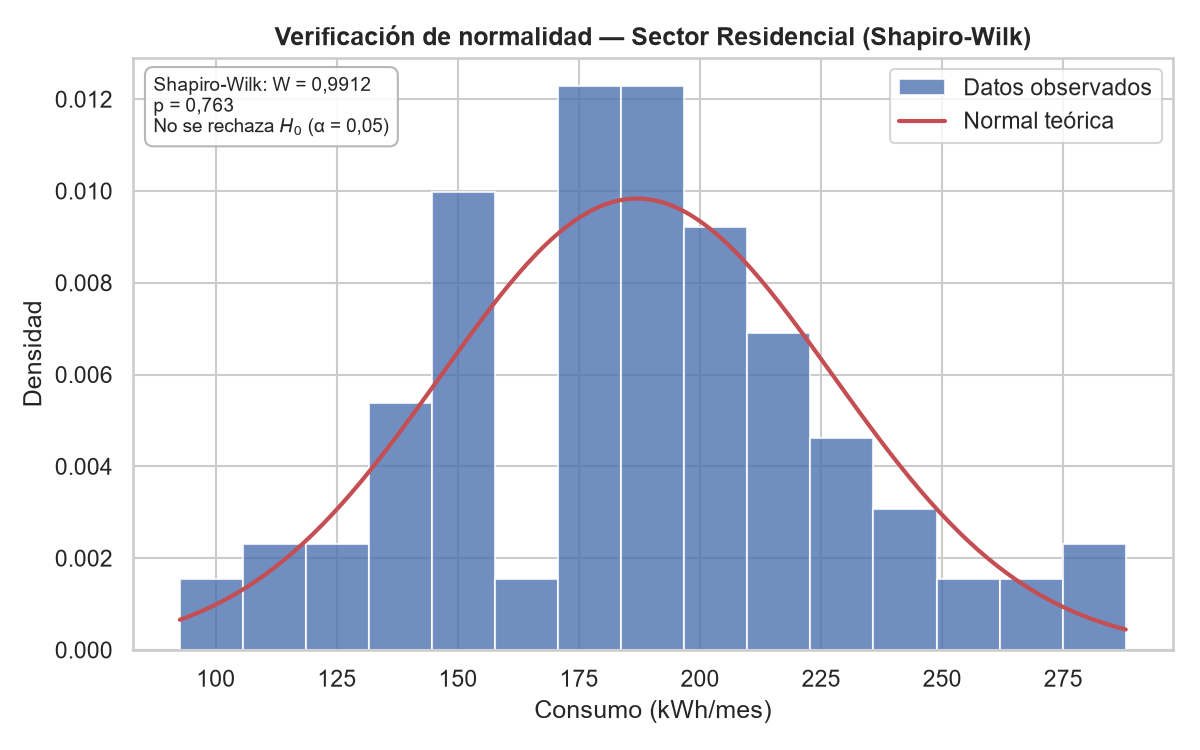
\includegraphics[width=0.99\linewidth]{assets/images/figures/python/hypothesis/histograma_normalidad.png}
            \caption{Verificación de normalidad del sector Residencial: histograma
            de la muestra con la densidad normal teórica superpuesta (Matplotlib)}
            \label{fig_normalidad}
        \end{figure}

        La Figura \ref{fig_normalidad} muestra un comportamiento compatible con 
        la normalidad. El valor $p=0,7628$ sin rechazar $H_0$, mientras 
        que la correspondencia entre el histograma y la distribución normal teórica 
        respalda gráficamente este resultado.

        \begin{strip}
            \centering
            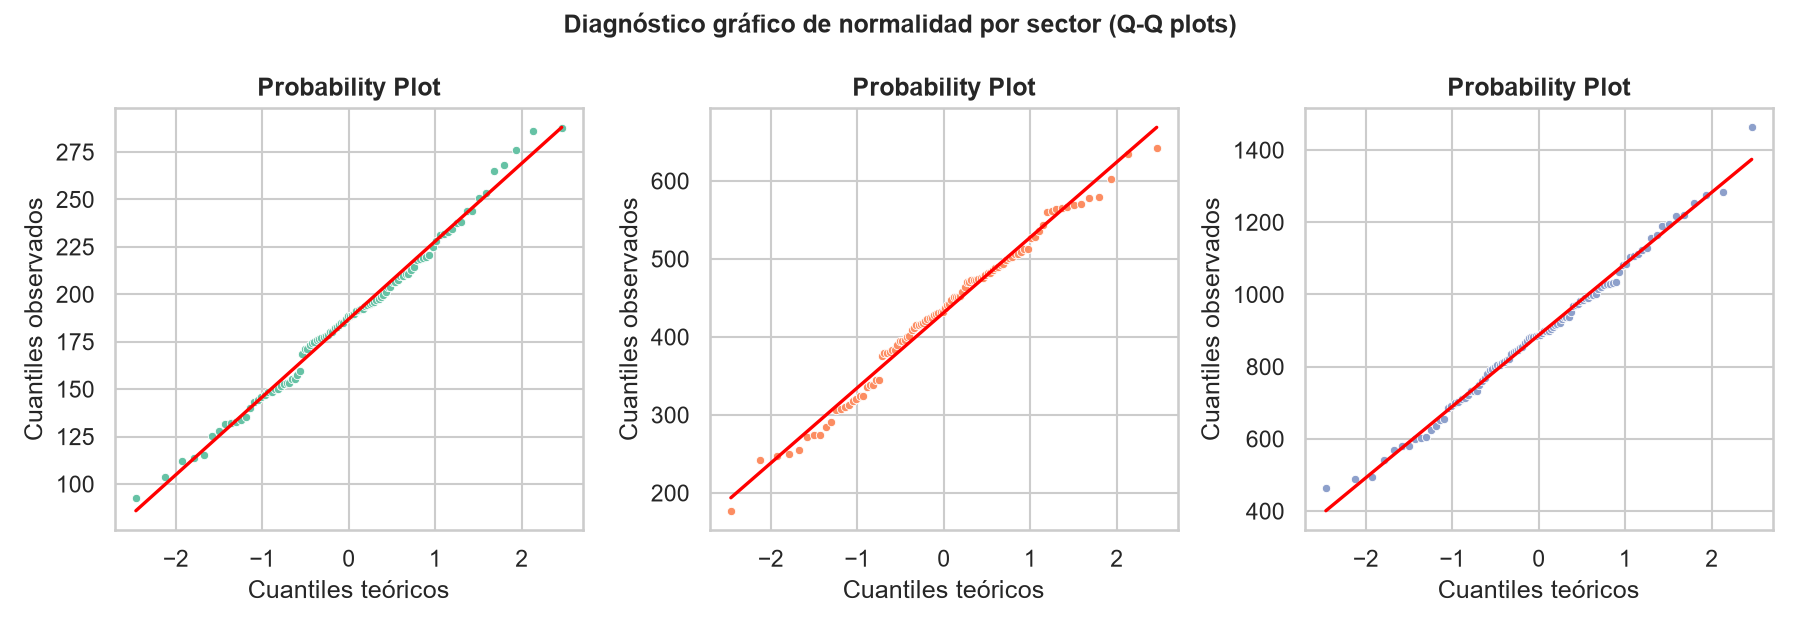
\includegraphics[width=0.92\linewidth]{assets/images/figures/python/hypothesis/qqplots_normalidad.png}
            \captionof{figure}{Diagnóstico gráfico de normalidad en los tres sectores mediante
            gráficos cuantil-cuantil (Matplotlib). Cada panel rotula el estadístico
            $W$ de Shapiro-Wilk y su valor $p$}
            \label{fig_qq}
        \end{strip}

        \clearpage

        El histograma representa el centro de la distribución, pero la
        Figura \ref{fig_qq} permite evaluar mejor las colas. En los tres
        sectores, los puntos siguen la diagonal teórica sin evidenciar asimetría
        ni colas pesadas, respaldando la normalidad tanto gráfica como
        analíticamente \cite{shapiro1965analysis}.

    \subsection{Comparación de medias}
        La Tabla \ref{ttest} compara el consumo promedio de dos sectores, el
        Residencial consume \textbf{187 kWh} al mes, mientras que el Comercial
        consume \textbf{431 kWh}, es decir, más del doble. Este salto de 244 kWh
        es tan consistente que ningún cliente residencial típico se parece a 
        ningún cliente comercial típico. El valor $p < 10^{-49}$ (prácticamente 
        cero) niega cualquier posibilidad de que esta diferencia sea fruto del 
        azar.

        \begin{table}[H]
            \centering
            \caption{Prueba t de Welch: Residencial vs. Comercial}
            \begin{center}
                \begin{tabular}{|l|c|c|c|c|c|}
                    \hline
                    \textbf{Grupo} & \textbf{$n$} & \textbf{Media} &
                    \textbf{$s$} & \textbf{$t$} & \textbf{$p$} \\
                    \hline
                    Residencial & 100 & 186,98 & 40,57 & \multirow{2}{*}{$-23{,}54$}
                    & \multirow{2}{*}{$2{,}3\times10^{-49}$} \\
                    \cline{1-4}
                    Comercial   & 100 & 431,30 & 95,54 & & \\
                    \hline
                \end{tabular}
                \label{ttest}
            \end{center}
        \end{table}

        Extendiendo el análisis a los tres sectores (Residencial, Comercial e
        Industrial), el ANOVA de la Tabla \ref{anova_tabla} rechaza la hipótesis
        de que consuman lo mismo. El estadístico $F=775,99$ es extremadamente
        grande e indica que la variabilidad entre sectores es 776 veces más 
        grande que la variabilidad dentro de cada sector. Con
        $p < 10^{-118}$, concluyendo que el sector determina el consumo.

        \begin{table}[H]
            \centering
            \caption{ANOVA de un factor sobre el consumo}
            \begin{center}
                \begin{tabular}{|l|c|c|c|c|}
                    \hline
                    \textbf{Fuente} & \textbf{SC} & \textbf{gl} & \textbf{$F$} &
                    \textbf{$p$} \\
                    \hline
                    Sector   & 25.298.262,0 & 2   & 775,99 &
                    $1{,}2\times10^{-118}$ \\
                    \hline
                    Residual & 4.841.297,4  & 297 & & \\
                    \hline
                \end{tabular}
                \label{anova_tabla}
            \end{center}
        \end{table}

        El sector explica el \textbf{83,9\%} de la variabilidad total del
        consumo, lo que evidencia una fuerte diferenciación entre los grupos 
        y el 16,1\% restante corresponde a variaciones individuales dentro de 
        cada sector. Esta alta proporción anticipa un aspecto relevante del 
        análisis posterior, porque al concentrar el sector y la mayor parte de 
        la variabilidad, otros factores pueden quedar parcialmente ocultos.

        \begin{table}[H]
            \centering
            \caption{Comparaciones múltiples de Tukey (IC del 95\,\%)}
            \begin{center}
                \begin{tabular}{|l|r|c|c|}
                    \hline
                    \textbf{Comparación} & \textbf{Dif.} & \textbf{IC 95\,\%}
                    & \textbf{$p$ ajust.} \\
                    \hline
                    Ind. $-$ Com. & $+456{,}4$ & [413,8 ; 498,9] &
                    $<0{,}001$ \\
                    \hline
                    Res. $-$ Com. & $-244{,}3$ & [$-286{,}9$ ; $-201{,}8$] &
                    $<0{,}001$ \\
                    \hline
                    Res. $-$ Ind. & $-700{,}7$ & [$-743{,}2$ ; $-658{,}2$] &
                    $<0{,}001$ \\
                    \hline
                \end{tabular}
                \label{tukey_tabla}
            \end{center}
        \end{table}

        El post-hoc de la Tabla \ref{tukey_tabla} confirma que las tres
        comparaciones son significativas y que ningún par de sectores 
        puede tratarse como equivalente. Las Figuras \ref{fig_boxplot} y 
        \ref{fig_medias} traducen ambas tablas: la primera muestra cajas 
        sin traslape con amplitudes crecientes, que sostienen a la vez el 
        rechazo del ANOVA y el de la homogeneidad de varianzas; la segunda 
        convierte el resultado de Tukey en intervalos de confianza que no 
        se solapan.

        \begin{figure}[H]
            \centering
            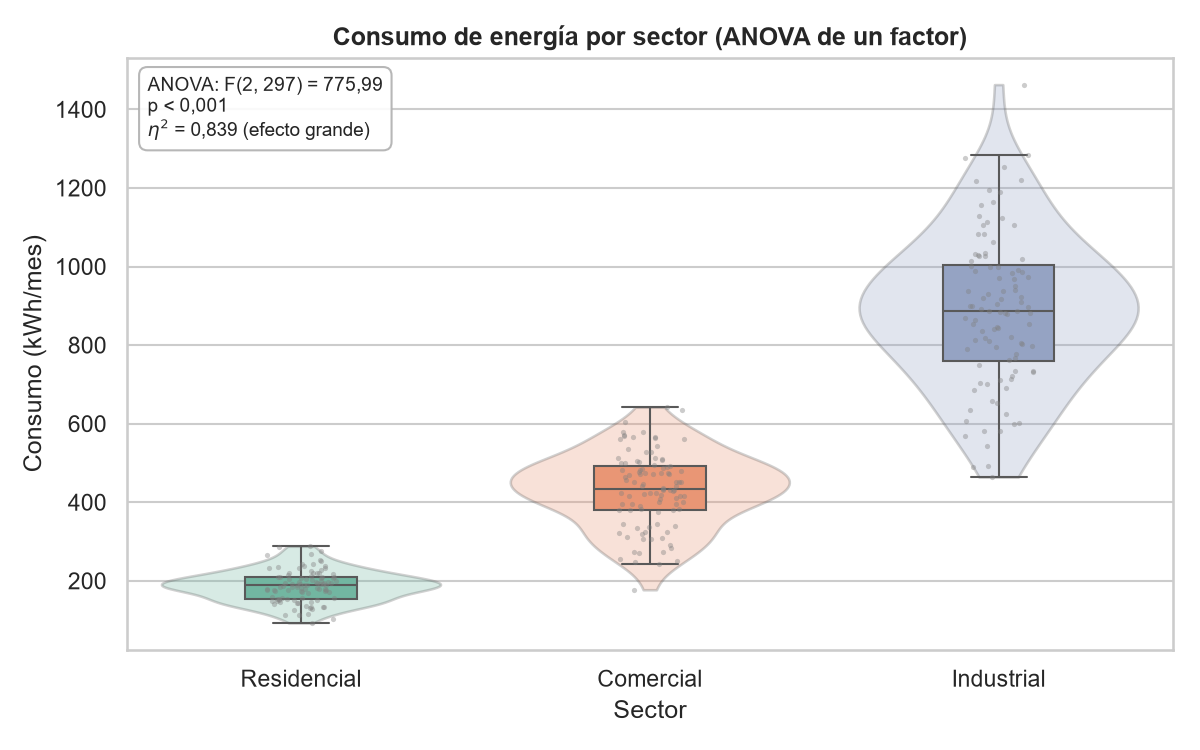
\includegraphics[width=1\linewidth]{assets/images/figures/python/hypothesis/boxplot_sectores.png}
            \caption{Distribución del consumo por sector: violín, caja e
            individuos superpuestos, con el resultado del ANOVA y su $\eta^2$
            rotulados sobre la propia figura (seaborn)}
            \label{fig_boxplot}
        \end{figure}

        \begin{figure}[H]
            \centering
            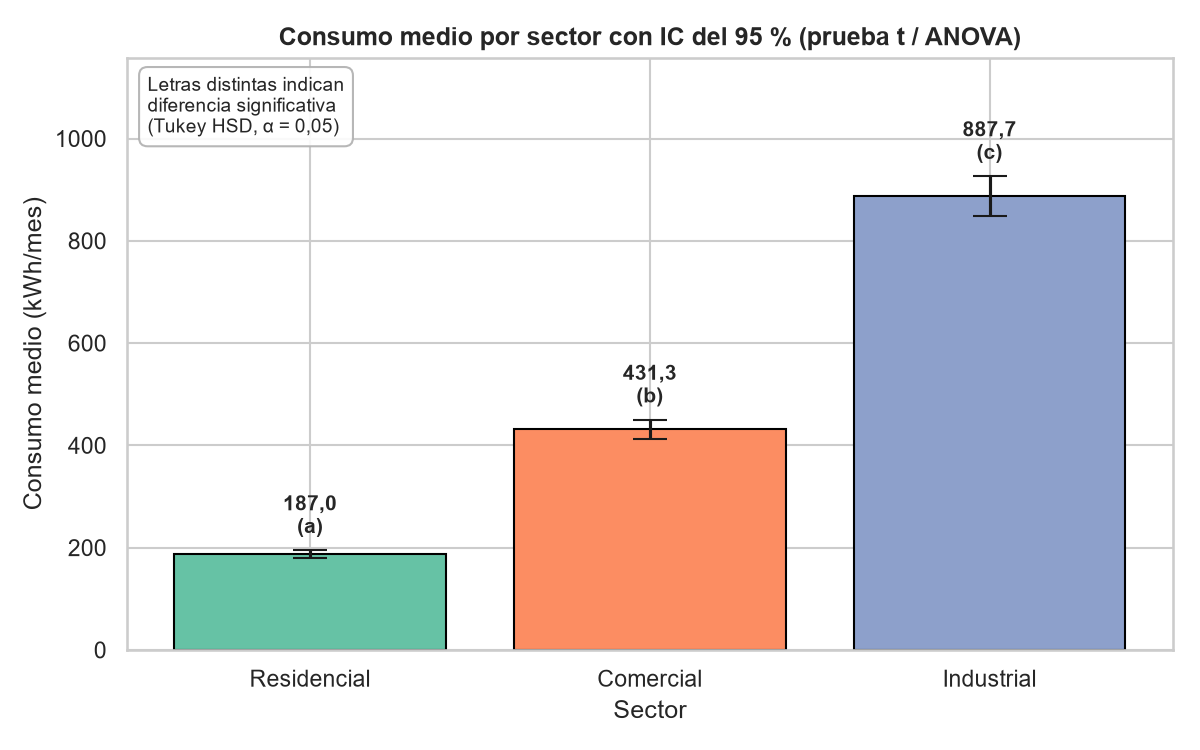
\includegraphics[width=1\linewidth]{assets/images/figures/python/hypothesis/medias_ic95.png}
            \caption{Consumo medio por sector con intervalos de confianza del
            95\,\%. Las letras (a), (b) y (c) codifican el post-hoc de Tukey:
            sectores con letras distintas difieren significativamente (Matplotlib)}
            \label{fig_medias}
        \end{figure}

    \subsection{Magnitud del efecto y potencia}
        \label{subsec_efecto_resultados}
        Los valores $p$ de las Tablas \ref{ttest} y \ref{anova_tabla} son tan
        extremos que dejan de ser informativos, con $n = 100$ por grupo indican
        que la diferencia existe, pero no cuánto vale. La Tabla \ref{efectos}
        cuantifica esa magnitud.

        \begin{table}[H]
            \centering
            \caption{Tamaños de efecto y potencia observada}
            \begin{center}
                \begin{tabular}{|>{\raggedright\arraybackslash}p{2.35cm}|c|c|l|}
                    \hline
                    \textbf{Medida} & \textbf{Valor} & \textbf{IC 95\,\%} &
                    \textbf{Lectura} \\
                    \hline
                    $d$ de Cohen (Res.--Com.) & 3,329 & [2,901 ; 3,757] &
                    Muy grande \\
                    \hline
                    $g$ de Hedges & 3,316 & --- & Muy grande \\
                    \hline
                    $\eta^2$ (sector) & 0,839 & --- & Muy grande \\
                    \hline
                    $\omega^2$ (sector) & 0,838 & --- & Muy grande \\
                    \hline
                    $f$ de Cohen (sector) & 2,286 & --- & Muy grande \\
                    \hline
                    Potencia ($t$ de Welch) & $>0{,}999$ & --- & Máxima \\
                    \hline
                    Potencia (ANOVA) & $>0{,}999$ & --- & Máxima \\
                    \hline
                \end{tabular}
                \label{efectos}
            \end{center}
        \end{table}

        Una $d=3,33$ indica una diferencia superior a tres desviaciones
        típicas entre Residencial y Comercial, muy por encima del umbral de
        efecto grande de 0,80 propuesto por Cohen \cite{cohen1988statistical}.
        El intervalo de confianza respalda esta magnitud y la corrección de
        Hedges apenas modifica la estimación. Asimismo, $\omega^2=0{,}838$ es
        prácticamente igual a $\eta^2=0{,}839$, lo que confirma que el 83,8\% de la
        varianza explicada no se debe al número de grupos. En conjunto, estos
        resultados evidencian un efecto genuinamente grande, no solo un
        resultado asociado al tamaño muestral.

        \vspace{10pt}

        Esta distinción se evidencia en la quinta hipótesis, donde con
        $n=300$ la ecuación (\ref{rdetectable}) establece $r_{\min}=0{,}161$
        como la correlación mínima detectable con una potencia del 80\%. El
        coeficiente global observado ($r=0,063$) queda por debajo de este umbral,
        mientras que el de Residencial ($r=0,595$) lo supera ampliamente, por
        tanto, la no significancia global no responde a un tamaño muestral
        insuficiente, sino a la baja magnitud de la correlación.

    \subsection{Robustez ante la heterocedasticidad}
        \label{subsec_robustez_resultados}
        El ANOVA de la Tabla \ref{anova_tabla} y el post-hoc de Tukey asumen
        varianzas iguales, supuesto que la Tabla \ref{supuestos} rechaza. La
        Tabla \ref{robustez} repite ambos contrastes con los procedimientos que
        no lo exigen.

        \begin{table}[H]
            \centering
            \caption{Contraste clásico frente a su versión robusta}
            \begin{center}
                \begin{tabular}{|l|c|c|c|}
                    \hline
                    \textbf{Procedimiento} & \textbf{$F$ / dif.} &
                    \textbf{gl} & \textbf{$p$} \\
                    \hline
                    ANOVA clásico & 775,99 & 2 ; 297 & $<0{,}001$ \\
                    \hline
                    ANOVA de Welch & 830,22 & 2 ; 156,1 & $<0{,}001$ \\
                    \hline
                    Tukey: Ind.$-$Res. & $+700{,}70$ & 297 & $<0{,}001$ \\
                    \hline
                    G.-Howell: Ind.$-$Res. & $+700{,}70$ & 107,5 & $<0{,}001$ \\
                    \hline
                    Tukey: Com.$-$Res. & $+244{,}33$ & 297 & $<0{,}001$ \\
                    \hline
                    G.-Howell: Com.$-$Res. & $+244{,}33$ & 133,6 & $<0{,}001$ \\
                    \hline
                    Tukey: Ind.$-$Com. & $+456{,}37$ & 297 & $<0{,}001$ \\
                    \hline
                    G.-Howell: Ind.$-$Com. & $+456{,}37$ & 143,8 & $<0{,}001$ \\
                    \hline
                \end{tabular}
                \label{robustez}
            \end{center}
        \end{table}

        La Figura \ref{fig_forest} muestra que Games-Howell estrecha el intervalo 
        entre Comercial y Residencial, pero lo amplía en las comparaciones con
        Industrial, el grupo más disperso. Tukey, al asumir un error estándar
        común, sobreestima la incertidumbre en la primera comparación y la
        subestima en las otras dos.

        \begin{figure}[H]
            \centering
            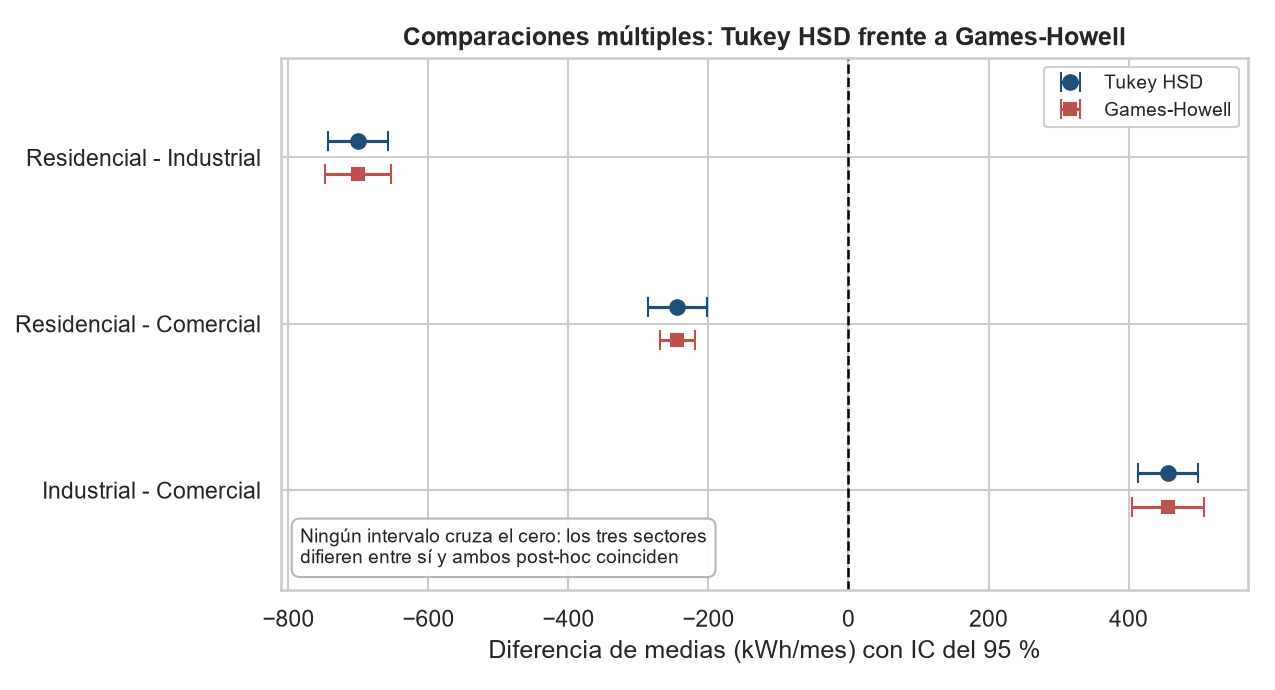
\includegraphics[width=1\linewidth]{assets/images/figures/python/hypothesis/tukey_forest.png}
            \caption{Comparaciones múltiples por pares: intervalos de confianza
            del 95\,\% de Tukey HSD frente a Games-Howell (Matplotlib)}
            \label{fig_forest}
        \end{figure}

        El ANOVA de Welch rechaza la igualdad de medias con un estadístico incluso 
        mayor que el clásico y las tres comparaciones de Games-Howell siguen siendo 
        significativas con intervalos que no cruzan el cero. El rechazo de la 
        homocedasticidad afecta a la precisión de cada intervalo, no a la decisión, 
        de modo que los resultados de las Tablas \ref{anova_tabla} y \ref{tukey_tabla} 
        pueden sostenerse tal como se reportan.

    \subsection{Relación entre temperatura y consumo}
        \label{seccion_regresion}
        La Tabla \ref{correlacion} presenta el coeficiente de Pearson calculado sobre 
        el conjunto completo y por separado, dentro de cada sector.

        \begin{table}[H]
            \centering
            \caption{Correlación temperatura-consumo por ámbito}
            \begin{center}
                \begin{tabular}{|l|c|c|c|l|}
                    \hline
                    \textbf{Ámbito} & \textbf{$n$} & \textbf{$r$} & \textbf{$p$} &
                    \textbf{Decisión} \\
                    \hline
                    Global      & 300 & 0,063 & 0,277 & No se rechaza $H_0$ \\
                    \hline
                    Residencial & 100 & \textbf{0,595} & $<0{,}001$ &
                    Se rechaza $H_0$ \\
                    \hline
                    Industrial  & 100 & 0,212 & 0,035 & Se rechaza $H_0$ \\
                    \hline
                    Comercial   & 100 & 0,183 & 0,069 & No se rechaza $H_0$ \\
                    \hline
                \end{tabular}
                \label{correlacion}
            \end{center}
        \end{table}

        La regresión global es $\hat{Y}=425{,}65+3{,}42,T$, con $R^2=0{,}004$, aunque 
        este resultado sugiere una relación prácticamente nula entre temperatura y 
        consumo, la ecuación (\ref{generador}) muestra que dicha conclusión no refleja 
        el comportamiento por sector. La Figura \ref{fig_regresion} presenta la nube 
        global sobre la que se obtiene este coeficiente.

        \begin{figure}[!htbp]
            \centering
            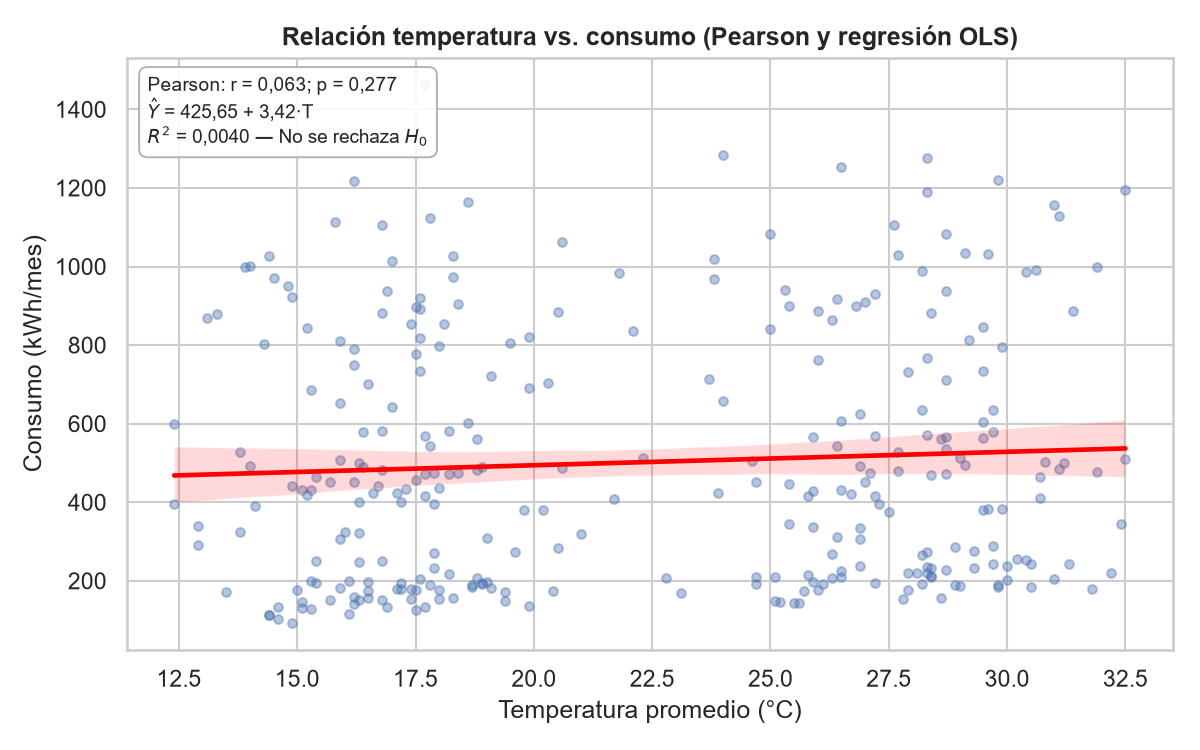
\includegraphics[width=1\linewidth]{assets/images/figures/python/hypothesis/regresion_temperatura.png}
            \caption{Relación temperatura-consumo sobre el conjunto agregado, con
            la recta de mínimos cuadrados, su banda de confianza y el resultado
            del contraste de Pearson rotulado (seaborn)}
            \label{fig_regresion}
        \end{figure}

        Acá se revela la contradicción, la nube se divide en tres franjas horizontales, 
        correspondientes a cada sector, mientras la recta global atraviesa las tres sin 
        representar adecuadamente a ninguna. La separación vertical entre franjas 
        responde al sector y no a la temperatura, dominando así la variabilidad 
        observada.